In a first step, we evaluated the covariance of the cryptocurrencies (BTC, ETH, XRP, LTC and the CMC200 index) and the 10 year treasury bond (TNX). The results are depicted in Figure \ref{fig:cov} below. We found small ($\leq$0.0021, ignoring covariance with oneself), positive values throughout. The magnitude  is not significant to interpret. Instead, we focus on the sign. All values are positive, indicating a positive relation of prices. Of most interest are the covariances of the 10 year tresury bond with the cryptocurrencies. These values are allocated along the bottom and right edge. The light pink color indicates very small values, close to zero. The covariance of two variables is close to zero if either both values are very small or if there is no relationship. Referring back to Figure \ref{fig:mean} we see that indeed the mean values of are variables are small ($<$0.003). We can therefore conclude that the risk-free rate and cryptocurrency returns are probably moving in the same direction.
\\


But what about the magnitude of the relation? This question can be answered with the Perason's correlation measure. The results are summarized below in Table \ref{fig:pearson}. We find a strong correlation between the various cryptocurrencies. This is not surprising. The different cryptocurrencies are substitutes of one another and most likely face the same demand trends. More interesting for our research question is the correlation between the 10yr treasury yield and the cryptocurrencies. The correlations are very weak. All of them are below 0.1 which according to \citet{corr} should be interpreted as a negligible connection. The highest correlation with the risk-free rate is achieved by the CMC 200 index, however also with very low magnitude (0.039). \\

The last part of the analysis consists of calcualting the Spearman's correlation coefficient. With this approach we try to control for potential non-linear relationships. However, the results are fairly similar to before. Especially, the correlation between the risk-free rate and the cryptocurrencies is still negligible.\\


\begin{figure}[!h]
    \centering
    \textbf{\caption{Covariance}}
    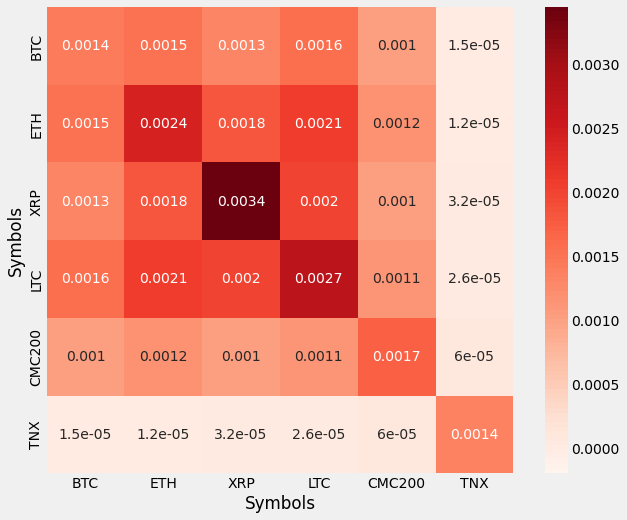
\includegraphics[width=0.8\textwidth,height=\textheight,keepaspectratio]{images/covariance_heatmap.png}
    \label{fig:cov} \\
    
    \note{\textit{Note.} Own representation.}
\end{figure} 

\begin{figure}[!ht]
    \centering
    \textbf{\caption{Pearson's Correlation}}
    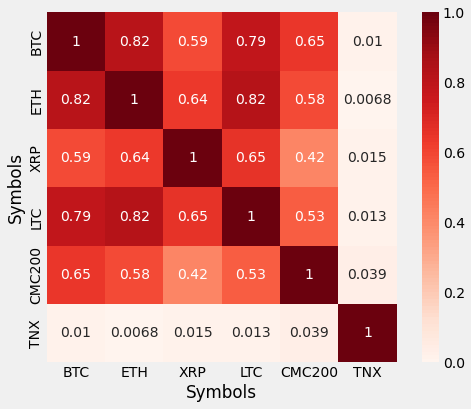
\includegraphics[width=0.8\textwidth,height=\textheight,keepaspectratio]{images/pearson_heatmap.png}
    \label{fig:pearson}\\
    
    \note{\textit{Note.} Own representation.}
\end{figure}